\appendix
\chapter{Przegląd praktyk stosowanych podczas prac nad projektem}
\label{cha:practices}

Celem niniejszego dodatku jest przedstawienie najważniejszych praktyk stosowanych przez autorów podczas wykonywania prac nad systemem GGSS. Poruszone zostały tematy organizacji pracy nad kodem w~zespole, dokumentacja projektu, czy też konwencje zastosowane w~celu uzyskania w~całym projekcie jednolitego kodu źródłowego.

\section{Wprowadzenie do problematyki}
Ze względu na zespołowy charakter przygotowanej przez autorów pracy inżynierskiej, w~trakcie jej wykonywania wprowadzone zostały praktyki mające na celu organizację i~koordynację współpracy. W~ramach platformy GitLab, wykorzystywanej przez CERN jako główne narzędzie do współpracy nad kodem, skorzystano z~szeregu funkcjonalności ułatwiających śledzenie postępów, jak i~zarządzanie projektem. Oprócz utworzenia zespołu, do którego został przypisany kod projektu oraz w~ramach którego odbywała się kolaboracja, wykorzystano:
\begin{itemize}
\item \emph{issue} - opis pojedynczego zadania/problemu. Zawiera podstawowe informacje, przypisaną osobę, etykietę, która oznacza obecny stan, termin wykonania oraz wagę
\item \emph{kanban board} - tablica kanban zawierająca wszystkie przypisane do projektu zadania. Kolumny takiej tabeli stanowią spersonalizowane do projektu etykiety. Pozwala na wysokopoziomowe zarządzanie projektem, sprawdzenie statusu, czy też łatwą zmianę etykiety przypisanej do zadań poprzez przeciągnięcie do odpowiedniej kolumny. % czy pokazac kanban board
\item \emph{merge request} - dedykowany widok do wprowadzania zmian wprowadzonych w~ramach kodu deweloperskiego do kodu produkcyjnego, który jest wykorzystywany do tworzenia i~dostarczania aplikacji
\item \emph{milestone} - kamień milowy, jednostka organizacyjna pozwalająca na grupowanie kilku zadań, które realizują większy cel. \emph{Milestone} śledzi przypisane do niego zadania, przewidywany czas zakończenia oraz wagę pozostałych do wykonania zadań.
\end{itemize}
W~trakcie wykonywania pracy inżynierskiej, szczególnie podczas początkowego etapu projektu, który odbywał się w~trakcie 3-tygodniowego wyjazdu do CERN, wyżej wymienione praktyki sprawdzały się bardzo dobrze.

\section{Motywacja do wprowadzenia zmian}
Ze względu na dobre sprawowanie się wyżej wymienionych praktyk w~trakcie pracy inżynierskiej postanowiono o~kontynuowaniu ich wykorzystania również w~trakcie pracy magisterskiej. Z~powodu nieregularnego aspektu pracy nad projektem, wykonywanie czynności zdalnie, lepsze poznanie środowiska, wykorzystywanych narzędzi oraz samej platformy GitLab postanowiono dostosować stosowane praktyki do nowych realiów. Dodatkowo bardzo ważną zasadą, biorąc pod uwagę zakończenie pracy nad projektem i~przekazanie go osobie odpowiedzialnej za dalsze utrzymanie, było odpowiednie udokumentowanie całego projektu. Wymagało się, aby możliwie proste było wprowadzanie zmian do systemu GGSS oraz sprawne, nieprzerwane działanie po zakończeniu pracy magisterskiej. Dlatego dostarczona dokumentacja musiała być obszerna oraz dobrze opisująca zastosowane rozwiązania. Dodatkowo biorąc pod uwagę mocny nacisk tejże pracy na część aplikacyjną projektu potrzebne było zdefiniowanie pewnych zasad pozwalających na ustandaryzowaną pracę z~kodem źródłowym aplikacji. Pozwoliło to na zachowanie pewnych konwencji w~całym projekcie, co zapobiegało różnicom w~kodzie między komponentami, a~co za tym idzie utrzymanie kodu oraz wdrożenie nowych osób do projektu jest znacznie uproszczone.


\section{Zmiana praktyk ze względu na nieregularność prac}

Prace nad systemem GGSS były kontynuowane, z~mniejszymi przerwami, od obrony pracy inżynierskiej. Natomiast ich charakter był nieregularny. Każdy z~autorów pracował nad systemem w~wybranych przez siebie godzinach. Ze względu na to wszystkie praktyki, które opierały się o~regularny czas pracy oraz przewidywanie czasu zakończenia danych zadań nie miały większego zastosowania. Postanowiono zatem zaprzestać przypisywania wag poszczególnym zadaniom. Oprócz wartości szacunkowej niewiele ona wnosiła w~trakcie wykonywania zadania, dodatkowo zdarzało się, że przybrane wartości różniły się od rzeczywistej wagi problemu, ponieważ często zadania wymagały w~pierwszej kolejności zgłębienia tematu, a~następnie określenia dokładnego rozwiązania problemu.

Zarzucono również praktykę wypełniania pola ,,termin oddania`` w~ramach tworzonych zadań. Ze względu na  wcześniej wspomnianą nieregularność czasu pracy nad projektem, informacja ta często nie zgadzała się z~rzeczywistym czasem zakończenia zadania. Dodatkowo nie była praktycznie w~ogóle potrzebna w~trakcie prac nad projektem ze względu na sposób formułowania zadań, które były możliwe do realizacji bez wpływu na pozostałe problemy. W~przypadku zadań, które wymagały koordynacji, czy też pracy od obydwu autorów, organizowane były spotkania online z~wykorzystaniem narzędzi takich jak Microsoft Teams, które pozwalały na tworzenie konferencji podczas których realizowane były wyżej wymienione zadania, czy też określane były ramy czasowe wykonania zadań od siebie zależnych. Sposób ten sprawdził się bardzo dobrze i~nie wymagana była dodatkowa koordynacja dla tego typu prac.

Rysunek \ref{fig:issue} przedstawia \emph{issue} utworzone według nowo ustalonych zasad. Brak jest przypisanego \emph{milestone}, czy też \emph{due date}. Natomiast ważne, wartościowe informacje, przydatne w~trakcie pracy nad projektem są wypełnione, tj.: rozbudowany opis pozwalający w~krótkim czasie zrozumieć o~co chodzi w~konkretnym zadaniu, osoby przypisane do \emph{issue} oraz etykiety oznaczające aktualny stan wykonania zadania, czy też jakikolwiek powód z~którego \emph{issue} nie zostało, bądź nie zostanie wykonane.

\begin{figure}[H]
    \centering
    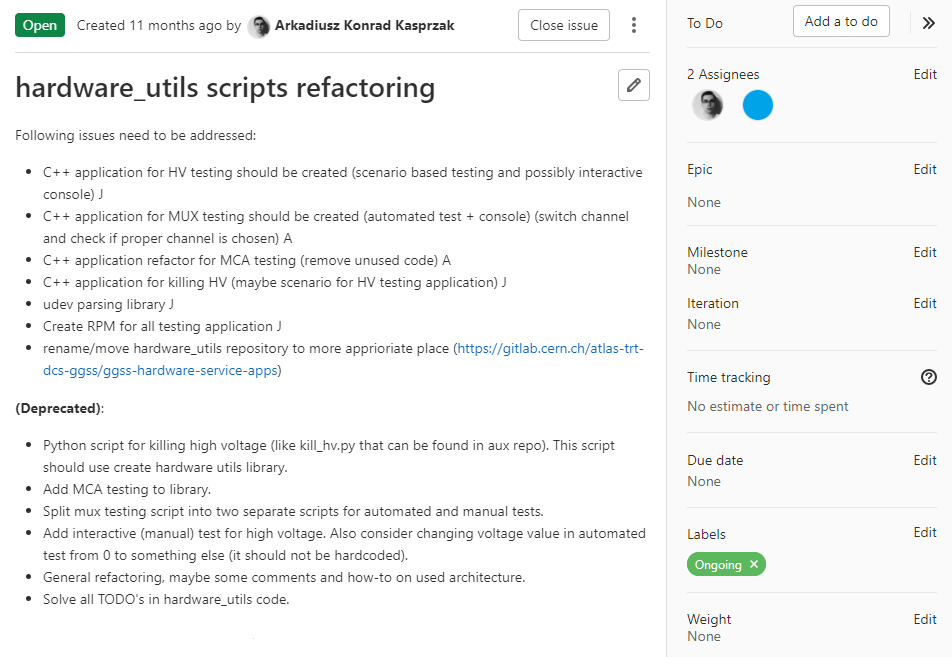
\includegraphics[width=\textwidth]{issue.png}
    \caption{Przykładowe \emph{issue} wg. nowo przyjętych praktyk}
    \label{fig:issue}
\end{figure}


\newpage
\section{Dokumentacja projektu}

%Wstepny tekst
Projekt GGSS ma być utrzymywany i~pozostać w~użyciu również po zakończeniu działań nad pracą dyplomową. Ze względu na to że rozwiązania wprowadzone do projektu były zarówno implementowane, jak i~projektowane przez autorów w~porozumieniu z~promotorem, posiadają oni niezbędną wiedzę na temat: powodów zastosowania pewnych rozwiązań, sposobu ich działania, sposobu korzystania z~nich, czy też zasad, które należy stosować w~trakcie rozwoju aplikacji. Ze względu na te czynniki dużo uwagi poświęcono przygotowaniu odpowiedniej dokumentacji pozwalającej na swobodną pracę z~projektem przez osoby, które ten projekt będą nadal utrzymywać.

% Dokumentacja na poziomie README
Dokumentacja w~postaci plików \emph{README} napisanych w~języku znaczników \emph{Markdown} jest dedykowana dla każdego z~repozytoriów. Zazwyczaj opisana jest w~niej zawartość danego repozytorium, sposób użycia tejże zawartości, jeżeli wcześniejsze przygotowanie zawartości jest potrzebne opisane są kroki, które należy w~takiej sytuacji poczynić. Dodatkowo w~wyżej wymienionych plikach opisane są wszelkie niuanse, czy też bardziej zaawansowane kwestie dotyczące zawartości danego repozytorium.

Rysunek \ref{fig:readme} przedstawia przykładowy plik \emph{README} dla repozytorium \emph{ggss-all} zawierającego infrastrukturę do budowy głównej aplikacji systemu GGSS. Wyżej wymieniony plik zawiera informacje o~przeznaczeniu repozytorium, wymaganiach potrzebnych do spełnienia w~celu uruchomienia infrastruktury budującej aplikację, krokach które należy podjąć, aby skorzystać z~tejże infrastruktury. Oprócz tego plik ten zawiera gotowe do użycia komendy, które można skopiować i~wkleić bezpośrednio do konsoli w~celu skorzystania z~infrastruktury. Plik ten zawiera również, a~co nie jest widoczne na rysunku, informacje o~sposobie uzyskania dostępu do kodu protokołu DIM, który jest wymagany do działania systemu GGSS.


Przygotowana w~ten sposób dokumentacja pozwala osobie praktycznie niezapoznanej z~projektem na skorzystanie z~infrastruktury i~przygotowanie gotowej do użycia, w~środowisku docelowym, aplikacji. Również powrót do projektu po dłuższej przerwie nie powinien powodować większych trudności.
\newpage
\begin{figure}[H]
    \centering
    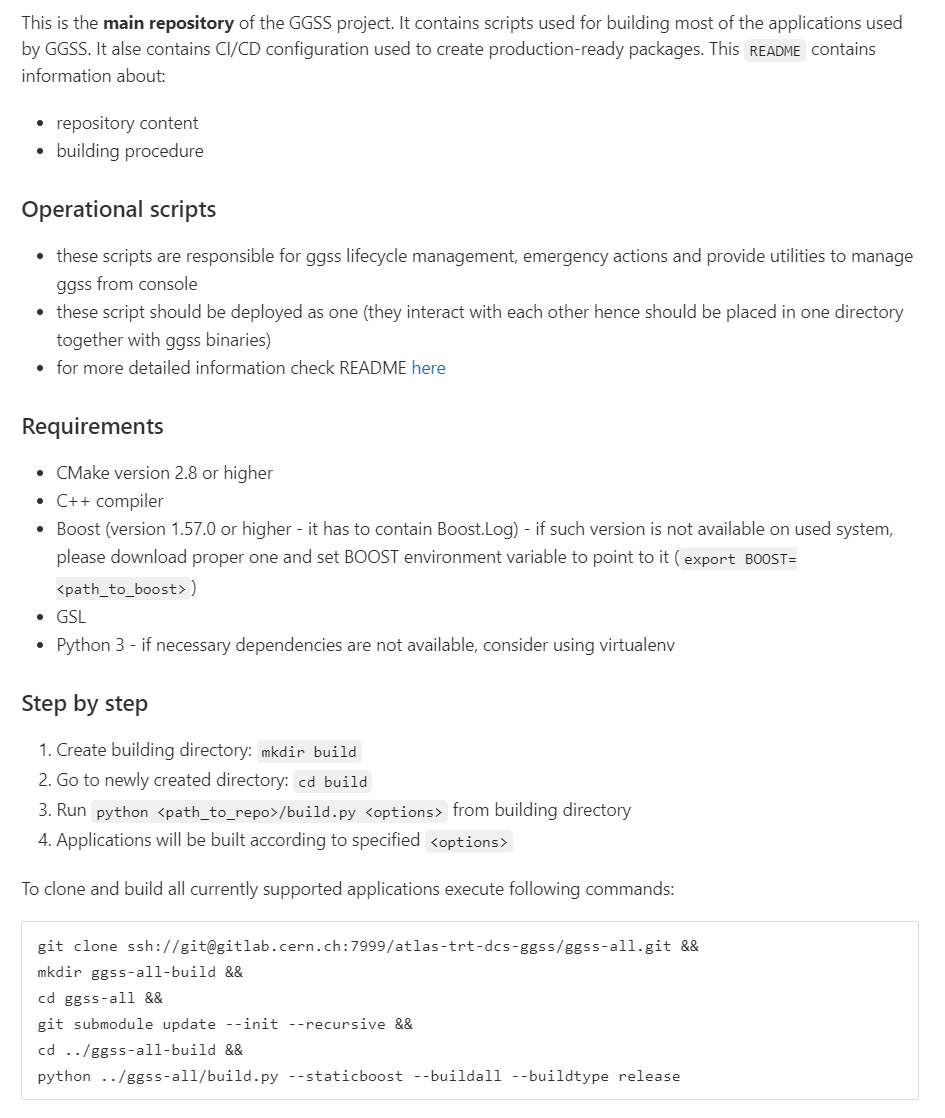
\includegraphics[width=\textwidth]{readme.png}
    \caption{Przykładowe \emph{README} w~ramach repozytorium \emph{ggss-all}}
    \label{fig:readme}
\end{figure} % zembedowac pdf

% Dokumentacja na poziomie kodu źrółowego
W~projekcie została zastosowana również dokumentacja na poziomie kodu źródłowego. Znajduje się ona między innymi: przed klasami, przed metodami, czy też na początku plików źródłowych. Dokumentacja ta stosuje format zgodny z~narzędziem Doxygen, co pozwoliło na jej ujednolicenie i~zwiększenie czytelności. Dzięki wcześniej wspomnianej zgodności możliwe jest wygenerowanie dokumentacji w~postaci plików HTML. Dokumentacja taka, w~celu jej przeczytania, wymaga jedynie aktualnej przeglądarki internetowej. W~celu pełnego wsparcia dokumentacji w~postaci plików HTML generowanych z~użyciem narzędzia Doxygen potrzebne było również dostosowanie infrastruktury służącej do budowania projektu, a~dokładnie plików CMake, dzięki czemu wygenerowane pliki \emph{make} posiadają moduły odpowiedzialne za obsługę wcześniej wspomnianej dokumentacji.

Listing \ref{lst:code_documentation} przedstawia przykładową dokumentację zgodną z~formatem wspieranym przez narzędzie Doxygen. Zawiera ona krótki opis dotyczący metody, następnie opis każdego z~parametrów przyjmowanych przez daną metodą oraz wartość zwracaną przez metodę. Informacje te są bardzo przydatne w~przypadku, gdy programista nie jest pewny, zważając na samą definicję metody, jej działania, parametrów wejściowych, czy też wyjścia. Opis taki rozwiewa częściowo wątpliwości i~pozwala w~poprawny sposób skorzystać z~wcześniej napisanego kodu.

\begin{lstlisting}[
    language=C++,
    caption={Przykładowy fragment kodu biblioteki \emph{fit-lib} wraz z~dokumentacją.},
    label={lst:code_documentation}
]
/**
 * \brief Class with naive peak finding algorithm implementation.
 */
class NaivePeakFinder : public PeakFinder
{
public:

    /**
     * \brief Computes initial peak position for Gauss fit.
     * \param fitData Data used for performing fit and finding peak position.
     * \param fitParams Structure with fit parameters (like fit range).
     * \return Calculated initial peak position.
     */
    double find(const std::vector<double>& fitData,
                const FitParams& fitParams) const override;
};
\end{lstlisting}

Rysunek \ref{fig:doxygen} przedstawia dokumentację jednej z~metod w~bibliotece \emph{fit-lib}. Zaprezentowana zawartość jest dokładnie taka sama, jak w~przypadku listingu \ref{lst:code_documentation}, natomiast przedstawiona w~bardziej przystępny sposób. Dokumentacja wygenerowana za pomocą narzędzia Doxygen świetnie nadaje się na udostępnienie zewnętrznym użytkownikom. Pozwala również w~łatwiejszy sposób przeglądać pełną dokumentację danego modułu bez potrzeby przeglądania kodu źródłowego.

\begin{figure}[H]
    \centering
    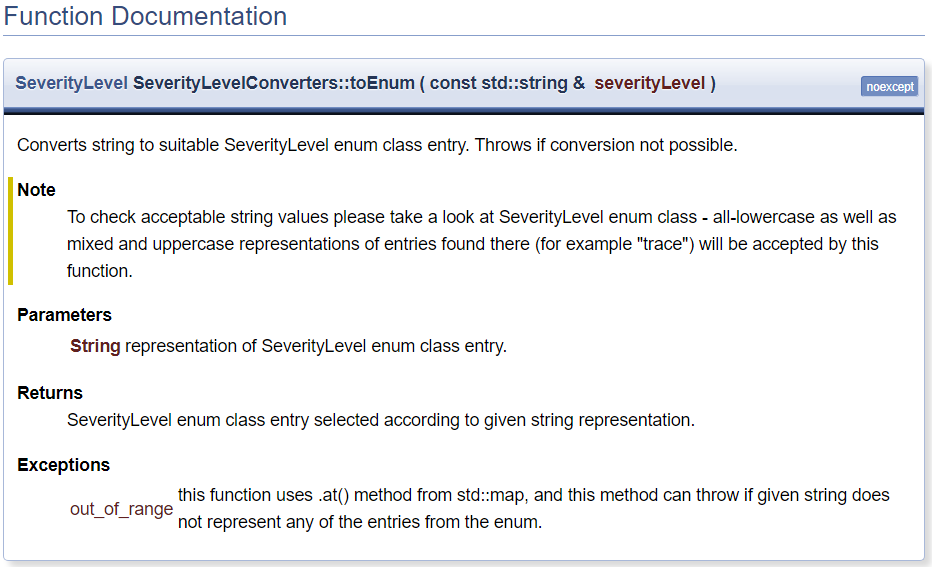
\includegraphics[width=\textwidth]{doxygen.png}
    \caption{Przykładowa dokumentacja metody w~bibliotece \emph{fit-lib} w~ramach projektu GGSS}
    \label{fig:doxygen}
\end{figure}

Ostatnim elementem dokumentacji zawartym w~projekcie są dokumenty \emph{how-to}. Napisane, podobnie jak pliki \emph{README}, za pomocą języka znaczników \emph{Markdown}, natomiast mają charakter globalny dla całego projektu - nie ograniczają się do jednego repozytorium. Dokumenty takie znajdują się w~repozytorium \emph{ggss-aux}. Opisane są tam krok po kroku bardziej zaawansowane aspekty pracy z~projektem GGSS, jak np.: sposób obsługi architektury wielopoziomowej opartej o~submoduły, czy też przygotowywanie wirtualnej maszyny do pracy jako GitLab Runner w~środowisku GitLab udostępnionym w~ramach infrastruktury CERN.

\section{Konwencja kodowania}
Ze względu na to, że w~trakcie pracy magisterskiej bardzo duży nacisk położono na część aplikacyjną projektu autorzy, jeszcze przed rozpoczęciem pracy nad kodem źródłowym, postanowili ustanowić konwencję kodowania, tak, aby na przestrzeni całego projektu GGSS utrzymać jednolity kod. Zasady, które zostały ustalony tyczą się nazewnictwa: klas, przestrzeni nazw, zmiennych, plików. Postanowiono wykorzystać, dobrze znane w~środowisku, systemy notacji ciągów tekstowych \emph{lower camel case} oraz \emph{upper camel case}. Ze względu na różnorodność możliwych rozszerzeń plików w~przypadku języka C++ postanowiono również ujednolicić ten aspekt. W~przypadku plików z~kodem źródłowym zastosowano rozszerzenia \emph{.cpp} oraz \emph{.h}. Ustanawiając konwencję kodowania postanowiono ograniczyć się do wyżej wymienionych aspektów, sposób projektowania architektury, podziału na foldery, klasy, etc. wewnątrz danego modułu pozostawiono bez większych obostrzeń. Oczywiście autorzy w~każdym z~dotkniętych miejsc stosowali dobre praktyki programistyczne oraz tak zwany \emph{clean code}, natomiast, ze względu na to, że w~większości przypadków prace nad projektem dotyczyły modyfikacji już istniejącego kodu oraz modułów była zachowana wcześniej zastosowana architektura.

